\documentclass[a4paper,11pt]{article} % Artículo porque a la hora de poner los títulos los enumera con 1., 2.,... sin embargo el report te los enumera así: 0.1., 0.2.,...
\usepackage[T1]{fontenc}
\usepackage[utf8x]{inputenc} % Esto hace que latex interprete la codificación del documento como utf-8 sin dar errores en las tildes
\usepackage[spanish]{babel} % Para poner el idioma en castellano(fecha,Índice...)
\usepackage{graphicx} %Para las imagenes
\usepackage{caption} %Para los textos de las imágenes
\usepackage{subcaption} % Para los textos de las imagenes tengan varios apartados
%Estas dos líneas (esta y la de abajo)ponen interlineado 1,5 excepto en notas a pie de página e igual algo más (que no sé)
\usepackage{setspace} % Paquete para interlineado.
\onehalfspacing % Interlineado a 1'5
%\usepackage{helvet}
%\renewcommand{\familydefault}{\sfdefault}
%\usepackage{uarial}
%\renewcommand{\familydefault}{\sfdefault}
\usepackage[nottoc,numbib]{tocbibind}

\usepackage[top=2.5cm, left=4cm, bottom=2.5cm, right=3cm]{geometry} % Para los márgenes

\usepackage{color} % Para poder poner las letras en color si es necesario
\usepackage[toc,page]{appendix} % Para poder poner los Anexos
\renewcommand{\appendixname}{Anexos} %Para cambiar de nombre los appendices por anexos
\renewcommand{\appendixtocname}{Anexos} %Para cambiar de nombre los appendices por anexos
\renewcommand{\appendixpagename}{Anexos} %Para cambiar de nombre los appendices por anexos
\newcommand*{\Appendixautorefname}{}

\usepackage[colorlinks=true, linkcolor=blue, citecolor=red, linktoc=page]{hyperref} % Para poner links
\usepackage{float}

% Páginas abajo a la derecha
\usepackage{fancyhdr}
\fancyhf{} % clear all header and footers
\renewcommand{\headrulewidth}{0pt} % remove the header rule
\rfoot{\thepage}

%\usepackage[]{adjustbox}

% Solución para colisiones entre hyperref y appendix
\usepackage{etoolbox} 
\makeatletter
\appto{\appendices}{\def\Hy@chapapp{Appendix}}
\makeatother
% % % % % % % % % % % % % % % % % % % % % % %
\usepackage{ccicons}
\usepackage{titlepage}
\begin{document} % Siempre hay que ponerlo
\pagestyle{empty}
\title{Anatomía de superficie: su representación pictórica en la muerte de Cristo}
\author{Nerea González Cordero}
\date{\today}
\maketitle % Para crear la portada
\newpage % Para salto de página

\textbf{Resumen}

La muerte a la largo de la historia ha sido temida, respetada, alabada o evitada en la medida de lo posible. Incluso en la actual sociedad, %a pesar de ser conscientes de que a todos nos llegará la hora de morir, 
sigue siendo un tema tabú.

Aún así, la muerte de Cristo en la cruz, siendo una gran desconocida, excepto por las distintas narraciones de los evangelios, es un tema muy recurrido en el arte, siendo ampliamente representada desde la antigüedad. Analizando varias obras se aprecia un recorrido histórico de la representación anatómica y de la muerte de Cristo, siendo éstas variables según las distintas creencias, percepciones sociales y religiosas e ideales de belleza de cada momento histórico.

Mediante el estudio de tres obras pictóricas y una escultórica se observan las variaciones en la anatomía %superficial
 de las figuras representadas, según el conocimiento anatómico de la época en la que se realiza cada una. %está realizada cada una de ellas. %que actúa como principal factor influyente. 
De aquí la importancia del análisis de la historia de la anatomía, sin la cual grandes obras %pictóricas y escultóricas 
no podrían haberse realizado.

Además, cada autor refleja de distinta forma la muerte de Cristo, obedeciendo a su propia conocimiento y a los principios de la época, desde un Cristo que no posee un rasgo de muerte en su apariencia, hasta otro que, en la búsqueda de un total realismo, refleja %lo más científicamente posible todas y cada una de las lesiones de este, además de 
todas las características presentes en la muerte. %de cualquier persona.

%Se pueden examinar desde las proporciones seguidas por el artista, hasta las características menos humanas y más divinas con las que algunos autores nos fascinan.

Asimismo, se pueden distinguir, en varias épocas, las diferentes percepciones de Cristo en cuanto a la representación de su gloria, como hijo de Dios y Dios, o su muerte, más humana, respectivamente.

%\vspace{10pt}

\textbf{Palabras Clave:}
Anatomía superficial, Cristo, muerte, crucifixión, obra de arte.

\vspace{10pt}

\textbf{Abstract}

Throughout history death has been feared, respected, or avoided if possible. Even in today's society it is still a taboo subject.

Even so, the death of Christ, being a great unknown except for all the accounts in the Gospels, is one of the more recurrent topics in art, being widely represented since antiquity. Analyzing some artworks it is noticeable a historical path of the anatomical representation and of the death of Christ, those of whom are changeable according to th different beliefs, social and religious perceptions and beauty ideals from each period of time.

By the study of three paintings and one sculpture, it is observable the variations on the surface anatomy of the represented figures, according to the anatomical knowledge in the epoch in which each is performed, %which acts as the main influential factor. 
Hence the importance of %analyzing 
the history of anatomy, without which large works of art%paintings and sculptures 
could not have been done.

In addition, each author reflects differently the death of Christ, in accordance with their own knowledge and the principles of the time, from a Christ who does not have any feature of death to another who, searching for total realism, reflects %as scientifically as possible %each and everyone of Christ injuries as well as 
all the features present in %anyone's 
death.

%It can be exhaminated from the proportions given by the artist until the less human features and the more divine ones some authors fascinate us with.

Furthermore, the different perceptions of Christ can be distinguished along the time, referring to his glory representation, as son of God and God, or even his death, more human, respectively.

%\vspace{15pt}

\textbf{Key words:}
Surface anatomy, Christ, death, crucifixion, artwork.
\tableofcontents % Para el Índice
\newpage

\pagestyle{fancy} % Empezar a numerar
\pagenumbering{arabic} % La numeración de las páginas, también se puede con números romanos {roman}

\section{Introducción} % Para los títulos
El arte podría definirse como una expresión de la creatividad humana que produce obras apreciadas por su belleza o emotividad y que es innata en el ser humano. Existe desde el origen del ser humano y  % (http://www.oxforddictionaries.com/definition/english/art)
a lo largo de los siglos ha ido evolucionando hasta el arte contemporáneo. Junto con las obras artísticas también se han ido transformando las representaciones anatómicas de obras pictóricas y escultóricas.

La anatomía de superficie es la ciencia que estudia las características anatómicas que pueden ser estudiadas mediante la vista y la palpación% (http://www.wikiradiography.com/page/Surface+Anatomy)
, es decir, la superficie del cuerpo. En el caso de la anatomía humana estudia desde las proporciones del cuerpo hasta puntos de referencia visibles en el exterior que están relacionados con órganos y partes internas, tanto en pose estática como en movimiento. % (http://www.princeton.edu/~achaney/tmve/wiki100k/docs/Superficial\_anatomy.html)

En este trabajo con anatomía de superficie me refiero a las estructuras corporales que se pueden identificar visiblemente, obviando aquellas estructuras que se pueden apreciar mediante la palpación, puesto que el trabajo tratará de la comparación de varias obras pictóricas. Me centraré exclusivamente en cuatro obras pictóricas: El Cristo crucificado de Velázquez, el Cristo crucificado con dos donantes de el Greco, el Cristo amarillo de Gauguin y el Cristo de San Juan de la Cruz de Dalí.

Primero comenzaré explicando las proporciones del ser humano y sus cambios en el arte durante distintos períodos de la historia, ya que las proporciones del cuerpo humano también son importantes en cuanto a anatomía de superficie se refiere.

Analizaré cada obra pictórica individualmente, centrándome en el contexto histórico y en la anatomía superficial que podemos discernir en cada obra. Después desarrollaré una conclusión acerca se las similitudes y las diferencias que estas obras tienen entre sí.

Además, fuera del trabajo se incluirán varios anexos:
%http://www.theodora.com/anatomy/surface\_anatomy\_index.html
\section{Objetivos}
Los objetivos a cumplir en este trabajo son varios. Existe un objetivo principal y otros secundarios.

El objetivo principal será identificar y estudiar la anatomía de superficie en el ecce homo. Para ello utilizaré varias obras diferentes cuyo análisis nos mostrará la agonía y muerte de Cristo representadas en diferentes épocas que, influenciadas a su vez por el contexto social y religioso, influyen en la pintura, en la anatomía y en la visión de Cristo de cada época.

Otros objetivos relacionados con éste son: afianzar los conocimientos anatómicos y desarrollarlos, analizar la historia de la anatomía que nos ha permitido llegar al conocimiento anatómico actual e identificar los cambios que se producen en el cuerpo en la agonía y en el momento inmediatamente después del fallecimiento y cómo lo representan en las distintas obras.

Además existen varios objetivos transversales que tienen que ver con la adquisición y la consolidación de conocimientos y habilidades para la realización del Trabajo de Fin de Grado (TFG). Me refiero a: la utilizacion de las bases de datos para conseguir información, el desarrollo de la capacidad de síntesis, el análisis crítico de la información encontrada y la elaboración adecuada y estructurada de un TFG.
\section{Metodología}
%TODO Hacer que el tiempo de esta sección esté acorde al utilizado anteriormente
En este trabajo con anatomía de superficie me refiero a las estructuras corporales que se pueden identificar visiblemente, obviando aquellas estructuras que se pueden apreciar mediante la palpación, puesto que el trabajo trata de la comparación de varias obras pictóricas. Me centro exclusivamente en cuatro obras pictóricas: El Cristo crucificado de Velázquez, el Cristo crucificado de El Greco, la lamentación sobre Cristo muerto de Mantegna % el Cristo amarillo de Gauguin 
y el Cristo de San Juan de la Cruz de Dalí.

%Primero comenzaré explicando las proporciones del ser humano y sus cambios en el arte durante distintos períodos de la historia, ya que las proporciones del cuerpo humano también son importantes en cuanto a anatomía de superficie se refiere.

Antes de examinar las obras y puesto que es el tema principal de las obras, mencionaré algunos puntos básicos acerca de la crucifixión y muerte de Cristo.

A continuación, analizaré cada obra pictórica individualmente, centrándome en el contexto histórico y en la anatomía superficial que podemos discernir en cada obra. También estudiaré las características presentes en las obras en relación a la muerte y la agonía de Cristo.

Por último, desarrollaré una conclusión acerca se las similitudes y las diferencias que estas obras muestran entre sí, así como del grado de fidelidad en relación a la época representada en ellas.

Además, fuera del trabajo se incluirán varios anexos:

\vspace{12pt}

Para redactar el documento se empleará un editor de texto llamado TexStudio, preparado para utilizar la herramienta de procesamiento de texto llamada Latex. Como fuentes de información principal en la realización del trabajo se utilizará el Encore, accesible mediante la página web de la biblioteca de la UPV-EHU, el cual está adscrito a numerosas bases de datos. Además, varios buscadores serán de gran utilidad en el ámbito que estudiaré: Google Academic y Google Art.

Una vez conseguida la información que podría ayudarme en la realización de mi TFG, desecharé aquella información que por distintas razones diverge de lo que se busca y me centraré en aquellos documentos, artículos y libros que considere de interés para el trabajo. Tras extensas lecturas y mucha síntesis lograré cumplir lo propuesto en los objetivos del trabajo.

Los anexos contenidos fuera del trabajo y los pies de página reflejarán información complementaria útil en la compresión del trabajo, que aún sin ser imprescindible, es una información que considero de interés.
\newpage
%\section{Muerte de Cristo}
La muerte de Cristo es una tema muy recurrido en la obra pictórica. En los siglos inmediatamente posteriores a la crucifixión no representaban tal cual al Cristo en la cruz, sino que lo hacían mediante otros símbolos y más tarde exclusivamente la cruz. Fue, sobre todo, a partir de la Edad Media (siglo V) cuando empezó a ser frecuente la imagen del Cristo crucificado.

Por otra parte, la iconografía cristiana varía de forma y estilo según las percepciones de la época artística en la que se desarrolla, en la que predomina un estilo determinado, pero en todas ellas ha tenido gran relevancia. De un joven imberbe se pasa a un hombre con barba. Ambas representaciones confluyen, pero artísticamente al final persiste la segunda. También se pasa de una visión de un Cristo triunfal a una visión más humana y menos divina de Cristo en el suplicio de la crucifixión.

Puesto que fue el emperador Constantino quien abolió la crucifixión en el siglo IV d.C, y no hay documentación ni representaciones acerca de ello hasta varios siglos después, es difícil saber cómo era en la época romana esta pena capital, que se utilizaba únicamente contra los peores delincuentes.

Se sabe que aunque ha habido distintas formas de crucifixión, los romanos del periodo comprendido alrededor del nacimiento y la muerte de Cristo utilizaban la cruz \textit{commisa}, la más frecuentemente representada, o la cruz \textit{immissa}, en forma de T (ver anexo \autoref{app:crosses}). Éstas estaban formadas por dos tablones de madera: un poste vertical que se insertaba en el suelo, que recibe el nombre de \textit{stipes} y un travesaño horizontal denominado \textit{patibulum}. A veces en la mitad del poste vertical se insertaba un bloque de madera que servía de asiento. También se utilizaba, aunque probablemente posteriormente al tiempo en el que vivió Cristo, un tablón que colocado a la altura de los pies ejercía de apoyo para éstos.

Dependiendo de la altura de las cruces éstas se dividían en la \textit{cruz humilde}, la más habitualmente usada, cuya altura era de unos dos metros y la \textit{cruz sublime}, tan alta que los pies del condenado se encontraban alrededor de un metro del suelo. Se cree que Cristo pudo haber sido crucificado en una de estas últimas ya que necesitaron una caña para poder acercarle la esponja con vinagre cuando estaba al borde de la muerte (Mt 27, 48; Mc 15, 36; Jn 19, 29). En este aspecto, muchas de las representaciones que podemos observar de crucifixiones de Cristo podrían ser correctas.

Diversas fuentes dejan claro que los Romanos utilizaban clavos para sujetar a los individuos crucificados a la cruz \footnote{Así como los evangelios atestiguan que Jesús fue clavado en la cruz, otros autores coetáneos se refieren también al uso de los clavos en la crucifixión. Ejemplos de ello son Séneca y Tranión. Además, las únicas reglas jurídicas que se conocen desde 1967 referentes a la crucifixión dan a entender que a los crucificados se les clavaba en la cruz.}. Además, la crucifixión variaba según la región y la inventiva del verdugo.

La creencia más extendida actualmente es la de que los clavos eran introducidos a la altura de la línea de flexión  de la muñeca, entre el cúbito y el radio y justo entre estos y los carpos o entre las dos filas de huesos metacarpianos. Se ha llegado a esta conclusión tras haber encontrado hallazgos arqueológicos de esta época que concuerdan con esta teoría y tras la realización de experimentos que apuntan a esta misma conclusión\footnote{El doctor Pierre Barbet realizó una serie de experimentos con cadáveres en los que se demostraba esta teoría.}. Anteriormente se creía que los clavaban en las manos porque así lo establece Juan en su Evangelio (Jn 20, 20-29), sin embargo ha de tenerse en cuenta que antiguamente la muñeca se encontraba en lo que se denominaba ``mano", que abarcaba hasta el brazo, lo que ha podido conducir a error durante siglos.

En cuanto a la técnica de clavado de los pies, no está claro si realizaban la inserción de los clavos juntando ambos pies y utilizado para ello un solo clavo o la fijación de éstos se llevaba a cabo por separado mediante dos clavos. Probablemente los calvos eran insertados entre el segundo y tercer metatarsiano. En las representaciones pictóricas se emplea tanto la imagen de Cristo crucificado mediante tres clavos como mediante cuatro.

Teniendo en cuenta las dificultades en el conocimiento de la crucifixión de Cristo es lógico pensar que en la mayoría de la iconografía referente al tema Cristo es representado según el gusto y estilo de cada autor claramente ubicado en su época.

% Enciclopedia moderna, 11: diccionario universal de literatura, ciencias, artes, agricultura, industria y comercio. Francisco de Paula Mellado (Pág:805-811)
% http://www.frugalsites.net/jesus/crucifixion.htm
% http://mb-soft.com/believe/text/crucifix.htm
% LA CRUCIFIXIÓN Laura RODRÍGUEZ PEINADO (en documentos del TFG)
% http://www.shroud.com/bucklin2.htm

Si existe debate acerca de si Jesús murió verdaderamente en la cruz \footnote{Algunos autores como Margaret y Trevor Lloyd Davies, los mayores defensores, consideran la posibilidad de que Jesucristo no muriese verdaderamente en la cruz. Otro ejemplo de esta hipótesis se encuentra reflejada en el libro \textit{42 días, Análisis forense de la crucifixión y la resurrección de Jesucristo}, de Miguel Lorente.}, mayor es el debate existente sobre la presunta causa de su muerte.

Existen varias teorías al respecto: 1) Embolia Pulmonar 2) Rotura cardíaca 3) Trauma de suspensión 4) Asfixia 5) Herida perforante fatal 6) Shock 7) Síncope fatal 8) Arritmia cardíaca 9) Coagulopatía inducida por traumatismos.

Todas estas hipótesis han sido analizadas en profundidad, no llegando, sin embargo, a la conclusión acerca de cuál es la real. Lo que está claro, sin embargo, es que Cristo padeció terribles sufrimientos, los cuales en conjunto pudieron conducirle a su muerte, que se produjo hacia las tres de la tarde tras solamente varias horas en la cruz.

% The Search for the Physical Cause of Jesus Christ's Death Author: W. Reid Litchfield Categories: God and Jesus Christ, Science Journal: 37:4 (en documentos de TFG)
% The crucifixion of Jesus: Review of hypothesized mechanisms of death and implications of shock and trauma-induced coagulopathy (en refworks)
\section{Análisis de la obra pictórica: Lamentación sobre Cristo muerto de Andea Mantegna}

Arte, estilo: Renacimiento italiano, quattrocento

Cronología: 1480

Lugar: Pinacoteca de Brera, Milán

Autor: Andrea Mantegna

Título: Lamentación sobre Cristo muerto

Función:

Contexto histórico: Andrea Mantegna realiza esta obra en pleno período humanista, el centro del mundo ya no es Dios o la religión, sino que el hombre pasa a ser el centro. Esto derivaría en ideas de libertad, rivalidad, competencia, que no hacen otra cosa que contribuir al gran avance que se da en el arte durante el Renacimiento en general.

Es durante esta época que los pintores comienzan a tomar importancia como artistas, no sólamente como meros técnicos. A partir de este momento empiezan a estudiar formas de hacer las obras más cercanas y reales para el espectador, se busca la consecución de una imagen con volumen, profundidad y dimensiones adecuadas. De esta manera se dan verdaderos progresos en la perspectiva o en las proporciones.

La obra analizada es, de hecho, una obra pionera en la perpectiva con la que representa a Cristo muerto. En épocas anteriores y en otras obras de la misma época en las que se representa a Cristo muerto, lo usual era contemplarlo de perfil. En la búsqueda de realismo en su obra el autor ladea la cabeza y los pies de la figura, eliminando, de esta forma, la estaticidad que le aporta la simetría del cuerpo, la cual también se ve anulada mediante las arrugas de tela que cubren la pelvis y las piernas de Cristo y las formas laxas del cuerpo.

Se trata de una obra dramática del cuerpo de Cristo muerto, antes de la resurrección y el triunfo sobre la muerte. Este dramatismo se percibe en la expresión tanto de la cara de la figura principal, como los rostros de aquellos que contemplan con horror la escena y se incrementa con los colores utilizados, de la misma gama cromática, la austera decoración del resto de la estancia, en la que solo vemos la lápida en la que se encuentra tumbado Cristo y la almohada en la que apoya la cabeza.

%http://www.arteespana.com/quattrocentoitaliano.htm
%http://www.arteespana.com/andreamantegna.htm
%http://www.artehistoria.jcyl.es/v2/obras/4376.htm
%http://educacion.ufm.edu/andrea-mantegna-lamentacion-sobre-cristo-muerto-oleo-sobre-tela-en-torno-a-1480-1490/
%http://cv.uoc.edu/~04_999_01_u07/percepcions/perc57.html
%Libro de Olatz

\vspace{12pt}
\textbf{Anatomía de superficie:}

Andrea Mantegna sorprende en su época con esta obra en la que Cristo se presenta en una perspectiva nunca antes vista, y con una figura de proporciones y anatomía exquisitas. Debido precisamente a la perspectiva en la que se encuentra la figura no es fácil discernir el modelo proporcional que sigue, aunque si es apreciable la armonía en la proporción de la figura, con una cabeza adecuada al tamaño del resto del cuerpo.

En esta obra se aprecia de manera sublime la muerte de Cristo. La laxitud de los músculos de las extremidades y la lividez que presenta el cuerpo nos da una idea bastante acertada de la imagen de un cadáver. La palidez amarillenta con la que el autor refleja el cuerpo y los tonos grisáceos incluso amoratados hacen visible lo que se denomina el \textit{pallor mortis}. Esta es una de las fases que acontece a nuestro cuerpo una vez el corazón deja de bombear sangre y, por tanto, esta no llega a los capilares, produciendo una palidez cadavérica. Una vez la sangre deja de circular tiende a por gravedad a dirigirse a la parte baja del cuerpo, que en el caso de la figura de la obra sería en su zona dorsal. En la obra se aprecian zonas más oscuras que podrían coincidir con estas zonas amoratadas del \textit{livor mortis}, pero podrían, de igual manera, tratarse de la propia sombra que proyecta la figura.

Se contemplan los orificios creados por los clavos en primer plano, tanto en los pies como en las manos, representados con gran realismo por el autor. Se pueden observar estos según las creencias de la época en las palmas de las manos, en lugar de a la altura de las muñecas, donde de acuerdo con la creencia actual, eran introducidos.
Las heridas, tanto las originadas por los clavos como la producida por la lanza, se encuentran limpias y sin una gota de sangre. Tanto es así que la del costado derecho apenas es visible en la perspectiva de la figura.

Se puede apreciar sin esfuerzo el volumen de las distintas partes del cuerpo, que el autor plasma duramente, casi a modo escultórico. 

Se percibe la laxitud de todos los músculos del cuerpo muerto, pudiendo, además, observar estructuras que en obras tan antiguas no solían aparecer, como son las plantas de los pies, donde apreciamos diversas estructuras anatómicas: el arco plantar, caramente definido y el calcáneo y las cabezas de los metatasianos, que están cubiertos por grasa subcutánea que sirve de almohadillamiento.

También se perfila de forma aparente la caja torácico, tras un vientre hundido, que hace notable el borde costal inferior. Y anunque las estructuras no están claramente precisadas se puede intuir, debido al vientre hundido, la espina ilíaca en ambos costados de la pelvis.

Las extremidades superiores caen inertes a ambos lados de la figura, con cierta flexión en las articulaciones del codo, muñeca, metacarpofalángica e interfalángicas probablemente debido al \textit{rigor mortis}. Éste se define como la rigidez que adquieren los musculos tras varias horas de la muerte debido a cambios químicos en las células del cuerpo. Refiriéndome a este mismo proceso, he de mencionar la rigidez de las piernas, puesto que si tal caso no se diera los pies caerían laxos hacia los lados.



La espalda se encuentra erguida, los músculos que se encargan de mantener esta postura son los principales erectores de la columna: los músculos del grupo iliocostal, los del grupo longuísimo y los del espinoso.

El músculo dorsal ancho, que además se puede apreciar en la obra, proviene de la espalda e inserta en el ángulo inferior de la escápula. Su tendón estrecho envuelve al músculo redondo mayor que forma el pliegue posterior de la axila. Ambos músculos junto con el pectoral mayor, el que además forma el pliegue anterior de la axila, elevan el tronco cuando los brazos se encuentran fijos, como es el caso de la figura examinada.

El músculo trapecio, cuya principal función es la elevación de la escápula, también se observa. El serrato anterior gira la escápula y, por tanto, junto con el músculo trapecio y el elevador de la escápula que la elevan hacen que la cavidad glenoidea se oriente hacia arriba y adelante, como en la figura de la obra de Velázquez.
El deltoides, que se ve fácilmente redondeando y sustentando la articulación del hombro por su parte superior, es el principal abductor del brazo, ya que sigue el movimiento abductor que el músculo supraespinoso inicia, por lo que tiene gran relevancia en la posición de crucifixión en la que ambos brazos se encuentran en posición de abducción.

En el brazo se observan tanto el bíceps como el tríceps. El bíceps forma una prominencia en la parte anterior del brazo y se encarga de la supinación del antebrazo, la cual realiza con la ayuda del músculo supinador. El tríceps por su parte se encarga de la extensión de la articulación del codo. En este movimiento le secunda el músculo ancóneo, que no es visible en la figura de la obra analizada por encontrarse en la parte posterior del codo.

La mano se encuentra en posición de reposo en la que las articulaciones falángicas y metacarpofalángicas se encuentran ligeramente flexionadas. El músculo palmar largo contribuye sutilmente a la flexión de las articulaciones metacarpofalángicas, que es realizada fundamentalmente por los músculos flexores de los dedos.

Al tratarse de un individuo delgado y favorecido por la postura en que se encuentra (brazos estirados hacia los lados y hacia arriba) se puede intuir la caja torácico perfectamente. El borde costal inferior formado por las seis últimas costillas es fácilmente visible, al igual que la depresión en la que se encuentra el cuerpo del esternón y el contorno de algunas costillas (probablemente la cuarta, quinta, sexta y séptima).

En el abdomen se encuentran los músculos abdominales, que se pueden apreciar, aunque no muy marcados. Estos músculos forman una vaina fibrosa a cada lado de la línea media. Ambas vainas se unen en esta, formando la línea alba. También se divisa bastante bien la línea semilunar, que marca el borde lateral del músculo recto del abdomen cuya principal función en la figura es el mantenimiento de la postura erecta apoyando así a los músculos erectores de la columna.

El músculo mas superficial de los músculos laminares del abdomen es el oblicuo externo. Este entre la espina y la tuberosidad púbica gira sobre sí mismo y forma el ligamento inguinal. La depresión que suele haber a la altura de ese ligamento, y que suele ser más visible en hombre, se puede observar perfectamente en la obra pictórica.

La posición de las piernas, en las que la rodilla derecha de la figura se encuentran una en posición de extensión, mientras que la otra se encuentra ligeramente flexionada, colaboran varios músculos. Los encargados de la extensión son: el cuadriceps y los músculos del tracto iliotibial, y los de la flexión son: los músculos poplíteos y los gemelos. Al estar de pie soportando el peso sobre una pierna, el lado de la pelvis que no soporta el peso se eleva. Esta acción está realizada por los glúteos medio y menor y deja a la vista la espina ilíaca del lado derecho.
La rótula o patella se puede apreciar, al igual que la tuberosidad tibial, sobre todo en la rodilla flexionada.

Los pies se encuentran apoyados en una tabla, soportando el peso del cuerpo, y se ubican en paralelo entre ellos ligeramente separados anteriormente, con un clavo en cada dorso y sangre que emana de la herida. En la parte anterior de éstos, los dedos se encuentran relajados.

%\section{Análisis de la obra pictórica: Cristo crucificado de el Greco}

Arte, estilo: Manierismo

Cronología: Hacia 1590-1596

Lugar: Museo de Cleveland

Autor: El Greco

Título: Cristo crucificado 

Función:
% http://www.ctv.es/USERS/ags/00013_mm.htm

Anatomía:
\section{Análisis de la obra pictórica: Cristo crucificado de Velázquez } 

Arte, estilo: Barroco

Cronología: 1632

Lugar: Museo del Prado, Madrid, España

Autor: Diego Velázquez

Título: Cristo crucificado

Función: Aunque se encontraba en el Convento de la encarnación de San Plácido, no está claro donde estuvo los primeros años tras su realización ni la función específica que desarrollaba. Posteriormente se tiene constancia de que estuvo en la sacristía de este convento hasta alrededor del 1804, año en el que Godoy lo compra al convento. Pasa después por distintas manos, llegando finalmente al Museo de Prado en 1829, donde permanece actualmente. % El Cristo crucificado de velazquez, trasfondo histórico religioso. % http://www.museodelprado.es/coleccion/galeria-on-line/galeria-on-line/obra/cristo-crucificado-1/

Contexto histórico: La realización de esta obra tiene lugar en la atmósfera religiosa y social de la contrarreforma. Este es el motivo principal por el cual durante esta época predominan las obras de carácter religioso como esta de Velázquez.

En esta obra Velázquez aplica los conocimientos que adquiere en su viaje a Italia, los cuales se pueden observar en la realización estructurada y detallada de la anatomía de Cristo.

Aunque en las primeras representaciones de la crucifixión de Cristo éste está clavado mediante cuatro clavos, a partir del siglo XIII comienzan a ser más habituales los tres clavos. Sin embargo, Velazquez en su obra no sigue el estilo de su eṕoca, sino que sigue las recomendaciones de su maestro Francisco Pacheco en cuanto al número de clavos que mantienen a la figura clavada en la cruz. Por ello podemos observar los pies de Cristo apoyados en un subpedaneum, cuya utilización se cree posterior a la época de Cristo, al que se ensamblan mediante dos clavos. También podemos apreciar los clavos de las manos colocados en las palmas, en contra de la creencia actual de que se encontraban a la altura de las muñecas, siguiendo lo relatado en la Biblia.

Además, emplea los contrastes de luz de acuerdo a la corriente tenebrista, siguiendo seguramente a Caravaggio. Por ello vemos grandes contrastes entre la luz y las sombras de unas zonas del cuerpo y otras, como si la luz procediera de un foco fijo, que en el caso de este cuadro provendría de arriba a la izquierda. La oscuridad que rodea al Cristo, sin ningún espacio ni persona a su alrededor, hace que la escena produzca una sensación mayor de soledad, en el calvario que representa el cuadro.
% http://www.arteespana.com/velazquez.htm

\vspace{12pt}
\textbf{Anatomía de superficie:}

En esta obra Velázquez nos cautiva con una figura con una postura serena y de proporciones y anatomía estudiadas.  Responde a un modelo de siete cabezas y media. Su longitud con los brazos extendidos es igual a su altura y el ángulo que forman entre ellos es de 115º.

El autor, no se centra demasiado en la reproducción de la muerte de la figura. De hecho, aunque la cabeza de la figura caiga sobre su pecho, pudiendo sugerir la muerte de éste, tal y como apreciamos la músculatura de la espalda, brazos y piernas da la impresión de que todavía se encuentra con vida. Se podría pensar que en lugar de haber fallecido, el Cristo representado se encuentra en una posición de descanso tras el sufrimiento experimentado antes de la crucifixión. Los brazos se encuentran extendidos ambos lados del cuerpo y los músculos del brazo y de la espalda que contribuyen a ello están claramente contraídos y extendidos, contrariamente a lo que ocurriría si Cristo ya hubiese perecido, en cuyo caso la musculatura permanecería laxa y exánime.

Por la posición de las piernas, donde podemos apreciar que, al tener ambos pies apoyados, carga el peso sobre el lado izquierdo, flexionando la articulación de la rodilla de este lado e iclinando la cadera hacia el lado contrario ligeramente, es también evidente que Cristo no ha fallecido aún. El autor utiliza este ligerísimo contrapposto clásico como elemento embellecedor de la obra dejando de lado la indudable incapacidad de una persona crucificada y fallecida o al borde del fallecimiento para realizar esta acción.

Además, la figura no muestra la lividez típica de un cadáver, todo lo contrario, la figura posee el color de una persona totalmente sana, a pesar de la pérdida de sangre que Cristo debió experimentar durante su calvario. Otro detalle importante de la obra es la escasa sangre que emana de las heridas de Cristo: apenas varias gotas en las heridas de los clavos y aún menos en la herida de lanza que muestra en el costado derecho. Un rasgo de la obra que  manifiesta la muerte de Cristo, que como ya he dicho para nada está representada, es precisamente esta herida del costado, la cual en teoría fue realizada postmortem, como verificación de la muerte.

Una serie de músculos colaboran en la consecución de la postura en la que se encuentra la figura a analizar.

La espalda se encuentra erguida, los músculos que se encargan de mantener esta postura son los principales erectores de la columna: los músculos del grupo iliocostal, los del grupo longuísimo y los del espinoso.

El músculo dorsal ancho, que además se puede apreciar en la obra, proviene de la espalda e inserta en el ángulo inferior de la escápula. Su tendón estrecho envuelve al músculo redondo mayor que forma el pliegue posterior de la axila. Ambos músculos junto con el pectoral mayor, el que además forma el pliegue anterior de la axila, elevan el tronco cuando los brazos se encuentran fijos, como es el caso de la figura examinada.

El músculo trapecio, cuya principal función es la elevación de la escápula, también se observa. El serrato anterior gira la escápula y, por tanto, junto con el músculo trapecio y el elevador de la escápula que la elevan hacen que la cavidad glenoidea se oriente hacia arriba y adelante, como en la figura de la obra de Velázquez.
El deltoides, que se ve fácilmente redondeando y sustentando la articulación del hombro por su parte superior, es el principal abductor del brazo, ya que sigue el movimiento abductor que el músculo supraespinoso inicia, por lo que tiene gran relevancia en la posición de crucifixión en la que ambos brazos se encuentran en posición de abducción.

En el brazo se observan tanto el bíceps como el tríceps. El bíceps forma una prominencia en la parte anterior del brazo y se encarga de la supinación del antebrazo, la cual realiza con la ayuda del músculo supinador. El tríceps por su parte se encarga de la extensión de la articulación del codo. En este movimiento le secunda el músculo ancóneo, que no es visible en la figura de la obra analizada por encontrarse en la parte posterior del codo.

La mano se encuentra en posición de reposo en la que las articulaciones falángicas y metacarpofalángicas se encuentran ligeramente flexionadas. El músculo palmar largo contribuye sutilmente a la flexión de las articulaciones metacarpofalángicas, que es realizada fundamentalmente por los músculos flexores de los dedos.

Al tratarse de un individuo delgado y favorecido por la postura en que se encuentra (brazos estirados hacia los lados y hacia arriba) se puede intuir la caja torácico perfectamente. El borde costal inferior formado por las seis últimas costillas es fácilmente visible, al igual que la depresión en la que se encuentra el cuerpo del esternón y el contorno de algunas costillas (probablemente la cuarta, quinta, sexta y séptima).

En el abdomen se encuentran los músculos abdominales, que se pueden apreciar, aunque no muy marcados. Estos músculos forman una vaina fibrosa a cada lado de la línea media. Ambas vainas se unen en esta, formando la línea alba. También se divisa bastante bien la línea semilunar, que marca el borde lateral del músculo recto del abdomen cuya principal función en la figura es el mantenimiento de la postura erecta apoyando así a los músculos erectores de la columna.

El músculo mas superficial de los músculos laminares del abdomen es el oblicuo externo. Este entre la espina y la tuberosidad púbica gira sobre sí mismo y forma el ligamento inguinal. La depresión que suele haber a la altura de ese ligamento, y que suele ser más visible en hombre, se puede observar perfectamente en la obra pictórica.

La posición de las piernas, en las que la rodilla derecha de la figura se encuentran una en posición de extensión, mientras que la otra se encuentra ligeramente flexionada, colaboran varios músculos. Los encargados de la extensión son: el cuadriceps y los músculos del tracto iliotibial, y los de la flexión son: los músculos poplíteos y los gemelos. Al estar de pie soportando el peso sobre una pierna, el lado de la pelvis que no soporta el peso se eleva. Esta acción está realizada por los glúteos medio y menor y deja a la vista la espina ilíaca del lado derecho.
La rótula o patella se puede apreciar, al igual que la tuberosidad tibial, sobre todo en la rodilla flexionada.

Los pies se encuentran apoyados en una tabla, soportando el peso del cuerpo, y se ubican en paralelo entre ellos ligeramente separados anteriormente, con un clavo en cada dorso y sangre que emana de la herida. En la parte anterior de éstos, los dedos se encuentran relajados.

%El Cristo representado se encuentra crucificado en una cruz \textit{commisa} en cuya parte superior se ubica el cartel en el que se indica que es el Rey de los Judíos.

%En el cuadro se puede observar la parte izquierda de la cara, la parte derecha está cubierta por el cabello que cae sobre ella. En cuanto a aquello que podemos ver, se trata de una cara inexpresiva con barba que cubre parte de las mejillas y el mentón. Bajo esta barba se puede apreciar la forma del hueso de la manbíbula (cuerpo, rama y ángulo). La mucosa de los labios es apenas visible entre el vello, aunque sí se intuyen incluso la comisura labial izquierda. 

%La nariz se presenta en el centro de la cara de forma piramidal. La estructura de la nariz la proporcionan los huesos nasales que articulan entre sí, con el hueso frontal(por donde se une a la frente) y con el hueso maxilar (por el que se une  a las mejillas). La parte más prominente de la nariz es el cartílago nasal que separa las dos fosas nasales. Se aprecia el espacio del surco naso-labial, aunque éste no se ve directamente, porque al igual que el mentón, está cubierto de vello. Sin embargo, sí se distingue la aleta nasal izquierda y el septo nasal, a la vez que se puede intuir la narina izquierda de la nariz. Se puede también vislumbrar una pequeña arruga, la línea naso-labial. Se ve la prominencia de la mejilla, formada por el hueso cigomático. 

%Entre la nariz y la frente se encuentra una depresión denominada nasión. La frente, formada por la convexidad lisa del hueso frontal, apenas es visible puesto que está tapada por la corona de espinas. Sus bordes inferiores (arcos supraciliares) dan lugar al borde superior de cada órbita. Además estos dos arcos se unen mediante un puente denomindo gabela. Superficialmente a estas elevaciones se encuentran las cejas.

%Medialmente el globo ocular está limitado por los huesos maxilar y frontal que articulan entre ellos, lateralmente está limitado por los huesos frontal y cigomático e inferiormente por el hueso maxilar. El globo ocular izquierdo no es visible, solo se adivina debajo del párpado superior que lo cubre, en el que además se puede observar una pequeña arruga. Sí se puede vislumbrar las uniones medial y lateral entre los párpados superior e inferior, que limitarían la hendidura palpebral en caso de estar abiertos. En sus bordes se encuentran las pestañas, manifestadas en la obra mediante una línea más oscura en el borde de los párpados.

%Ambas orejas están tapadas por el cabello, por lo que sus partes no son visibles.

%El resto de la cabeza está formada por la bóveda craneal, la cual se insinua debajo del cabello. La cara lateral de la bóveda la componen los huesos frontal, parietal, occipital y temporal.
%El cuello no es visible, al estar la cabeza inclinada hacia abajo, ésta tapa las estructuras anatómicas del cuello.

%\vspace{12pt}

%En la imagen se puede observar el torso desnudo de Cristo crucificado, en el que se aprecian una serie de estructuras anatómicas. 

%Al tratarse de un individuo delgado se puede intuir la caja torácico perfectamente. Vislumbramos, a duras penas, la clavícula izquierda que articula con el esternón (manubrio) y la primera costilla, la derecha, no es visible, puesto que está tapada por el cabello. El borde costal inferior formado por las seis últimas costillas es fácilmente visible, al igual que la depresión en la que se encuentra el cuerpo del esternón y el contorno de algunas costillas (probablemente la cuarta, quinta, sexta y séptima), sobre todo las del lado derecho, ya que la sombra del propio cuadro nos  impide ver bien las del izquierdo. La escotadura esternal, también se puede intuir sobre la cara superior del manubrio, sin embargo, hay que dejarse llevar un poco por la imaginación, ya que, de nuevo la sombra del cuadro nos impide su correcta visualización. No se observa la apófisis xifoides, que está cubierta, por el recto anterior del abdomen, lo que se considera normal anatómicamente.

%En cuanto a los músculos podemos vislumbrar el pectoral mayor, que inserta en el borde interno de la clavícula, en los cartílagos de las seis costillas superiores y en el húmero, formando así el pliegue anterior de la axila, muy claro en la imagen, junto con el músculo deltoides, que se puede contemplar recubriendo la articulación del hombro. Lateralmente no se observan claramente los músculos. El serrato anterior que inserta en el borde anterior interno de la escápula, y en las ocho costillas superiores, junto con sus interdigitaciones con el músculo oblicuo externo podrían ser visibles en un individuo delgado y musculoso como el Cristo que representa este cuadro, sin embargo no es fácil de reconocer. Sí se puede apreciar el músculo dorsal ancho, proveniente de la espalda e insertado en el ángulo inferior de la escápula. Su tendón estrecho envuelve al músculo redondo mayor que forma el pliegue posterior de la axila. Este va desde el borde lateral de la escápula hasta el surco bicipital del húmero. El borde lateral de la escápula puede percibirse a través de la masa del redondo mayor.

%Los pezones se encuentran en el Cristo de la obra alrededor del cuarto espacio intercostal, lo que es anatómicamente correcto.

\vspace{12pt}

%En el abdomen, que delimita superiormente con el reborde costal, que como ya he dicho es claramente visible en esta obra, se encuentran los músculos abdominales, que se pueden apreciar, aunque no muy marcados. Estos músculos forman una vaina fibrosa a cada lado de la línea media. Ambas vainas se unen en esta, formando la línea alba. La figura no está suficientemente musculada para poder apreciar las tres inserciones tendinosas que se encontrarían encima del ombligo, a duras penas podríamos localizar una de ellas. Sí se divisa bastante bien la línea semilunar, que marca el borde lateral del músculo recto del abdomen.

%La espina ilíaca si se aprecia, sobre todo en el lado derecho, que es el lado hacia el que está ligeramente inclinada la cadera.

%El músculo mas superficial de los músculos laminares del abdomen es el oblicuo externo , pero como ya he comentado anteriormente no se ve claramente, y aunque sepamos que tiene que estar ahí, sus interdigitaciones con el serrato anterior no son visibles en el cuadro. Este músculo se inserta superiormente en las ocho costillas inferiores e inferiormente en la sínfisis de púbis, tuberosidad púbica, espina ilíaca anterosuperior y cresta ilíaca. Entre la espina y la tuberosidad púbica gira sobre sí mismo y forma el ligamento inguinal. La depresión que suele haber a la altura de ese ligamento, y que suele ser más visible en hombre, se puede observar perfectamente en la obra pictórica.

%\vspace{12pt}

%Las estructuras pélvicas no son visibles, debido a que el autor coloca encima un paño blanco con el que las tapa.

%\vspace{12pt}

%Las extemidades superiores se encuentran extendidas cada una hacia un costado de la cruz: Los músculos son visibles claramente.

%Antes de empezar con los músculos del brazo propiamente dichos, remarcaré algúno que se encuentra sustentando la articulación del hombro. El músculo trapecio sí se observa, este lateralmente se inserta en el tercio externo de la clavícula, el acromion y la espina de la escápula. Estas estructuras no son visibles anteriormente en la posición en la que se encuentra la figura analizada (brazos extendidos hacia los lados), sin embargo podemos apreciar un hueco en la unión de este músculo a las estructuras previamente citadas. El músculo que no nos deja ver esas estructuras es el deltoides, que también se ve fácilmente redondeando la articulación del hombro por su parte superior, cubriendo la epífisis proximal del húmero. Se inserta medialmente, al igual que el trapecio, en la clavícula, el acromion y la espina de la escápula y lateralmente en el tubérculo deltoideo de la cara lateral del húmero. Es el principal abductor del brazo por lo que tiene gran relevancia en esta posición.

%En el brazo se observan tanto el bíceps como el tríceps. El bíceps forma una prominencia en la parte anterior del brazo. Tiene dos cabezas, de las cuales la corta inserta en la apófisis coracoides y la larga en la cara superior de la fosa glenoidea de la escápula. Distalmente se inserta en la tuberosidad bicipital del radio, pasando por el medio de la fosa cubital.

%En ambos brazos podemos distinguir la fosa cubital. Esta está limitada superiormete por la línea que va desde la epitróclea hasta el epicóndilo del húmero, lateralmente por el músculo braquiorradial y medialmente por el pronador redondo.

%Los huesos de la articulación del codo suelen ser evidentes. En esta obra no se pueden distinguir claramente las distintas estructuras debido a la posición de los brazos (se verían mejor desde la cara posterior). Lo único que se aprecia de forma clara es la epitróclea del húmero.

%Los brazos se encuentran en total supinación y extensión. La extensión la realiza el tríceps junto con la contribución de los músculos del origen del extensor común. Y de la supinación se encargan el bíceps y el supinador.

%A la altura de las muñecas podemos observar las apófisis estiloides del cúbito y del radio, que en una persona un poco más gruesa no serían visibles. Además, se podrían intuir los tendones de los músculos del antebrazo que pasan a la mano. Cuando se flexiona la muñeca sobresalen tres tendones. El flexor carpi radialis se inserta distalmente en la base de los metacarpos 2 y 3, el flexor carpi ulnaris de inserta en el pisiforme y de allí en el ganchoso y en la base del quinto metacarpiano.

%Las venas, tanto cefálica como basílica suelen se visibles en mayor o menor medida en hombres jóvenes, delgados y en cierta medida musculados, no obstante, no han sido dibujadas por el artista en esta figura.

%En la obra se puede apreciar la palma de la mano derecha, aunque parcialmente, pues en ella se encuentra clavado el clavo a la cruz. Además los dedos se encuentran ligeramente flexionados, por lo que podemos vislumbrar las articulaciones interfalángicas en ellos. El metacarpiano del primer dedo también lo podemos distinguir en el cuadro. Este posee más movilidad que el resto de los metacarpianos, que además no son visibles en el cuadro, puesto que están tapados por los músculos de la palma.

%En la mano izquierda básicamente se observan las mismas estructuras que en la derecha. Pero además podemos percibir la denominada tabaquera anatómica. La tabaquera anatómica es una concavidad presente en la cara lateral de la muñeca, que se evidencia más al extender el primer dedo. Está limitada por varios tendones: el abductor largo del pulgar, que se inserta distal al primer metacarpiano; el extensor corto del pulgar, que se inserta en la falange proximal del pulgar; y el extensor largo del pulgar, que inserta en la falange distal del primer dedo.

%En las palmas de ambas manos se observan tanto la eminencia tenar, como la hipotenar.

%La emnencia tenar se denomina al abultamiento lateral presente en la palma de la mano, a la altura del primer dedo. Está formada por los músculos cortos del pulgar: los músculos abductor, flexor y oponente del pulgar.

%La eminencia hipotenar se denomina al abultamiento medial de la palma de la mano a la altura del quinto metecarpiano. Está formada por el abductor, el flexor y el oponente del meñique.
%Podemos apreciar cierta flexión en las articulaciones metacarpofalángicas, la cual es producida por los músculos lumbricales que se encuentran entre los dedos. Los dedos también mantienen cierta flexión, producida esta por los tendones de los flexores superficial y profundo de los dedos.

% \subsubsection{Visión anterior del antebrazo}
% El músculo pronador se inserta sobre la cara anterior de la epitróclea y en la región central del radio. Es un pronador del antebrazo. Los tendones de los músculos flexor carpi radialis, palmar mayor, flexor superficial de los dedos y flexor carpi ulnaris pasan a la mano. Son también flexores débiles del codo.
% El músculo braquiorradial se inserta proximalmente  en los dos tercios superiores de la cresta supracondílea del húmero y distalmete en la cara lateral de la epífisis distal del radio. Este músculo prona o supina el antebrazo.

%El pisiforme es visible, así como el tubérculo del escafoides.

%\vspace{12pt}

%Podemos apreciar claramente la masa muscular de las estremidades inferiores, ya que estas se encuentran al descubierto. Sin embargo no es así de fácil distinguir los músculos específicos que producen esta masa muscular.

%Podemos intuir a duras penas por donde pasa el músculo sartorio, que que inserta en la espina ilíaca y en la superficie subcutánea medial de la parte superior de la tibia. Así mismo se podría señalar el músculo cuadriceps, músculo principal de la cara anterior del muslo, junto con sus tres cabezas superficiales: vasto externo, vasto interno y recto anterior, no el vasto intermedio, que va bajo el recto anterior.

%Los músculos pectíneo, psoas-ilíaco y recto interno no son visibles pues están tapados por el paño blanco que también tapa las estructuras pélvicas. No son claramente apreciables otros músculos superficiales como el tensor de la fascia lata (que inserta en la cara externa del ilion y en la tibia, formando el tracto iliotibial al unirse con el glúteo mayor), que esta situado en el lateral del muslo, superficialmente al trocánter mayor del fémur.

%El músculo cuadriceps forma en su parte inferior el "ligamento patelar" que recubre la rótula y se inserta en la tuberosidad tibial. En una figura delgada como esta la rótula o patella se puede apreciar, al igual que la tuberosidad tibial, aunque son más fáciles de apreciar en la flexión de la rodilla.

%El resto de estructuras de la rodilla no son apreciables, aunque se pueden intuir: condilos femorales, ligamentos de la articulación, tubérculo adductor del fémur, retináculos rotulianos medial y lateral...

%La rodilla derecha de la figura se encuentran una en posición de extensión, mientras que la otra se encuentra ligeramente flexionada. Los músculos encargados de la extensión son: el cuadriceps y los músculos del tracto iliotibial, y los de la flexión son: los músculos poplíteos y los gemelos.

%Podemos apreciar la tibia desde la tuberosidad tibial hasta el maleolo medial, en su recorrido subcutáneo.

%La masa muscular que se puede visualizar la conforman varios músculos. El músculo tibial anterior se encuentra en el lateral de la pierna y es el único de los cuatro músculos que inserta en la tibia. Además tiene un tendón distal que pasa hacia la base del primer metatarsiano. Otros músculos que forman esta masa muscular son el extensor largo del dedo gordo y el extensor largo de los dedos. Sin embargo también se pueden apreciar en la cara lateral músculos que en principio forman parte de la parte posterior: el sóleo y una de las cabezas del gemelo (superior al sóleo), que se unen para formar el comunmente denominado tendón de aquiles. Más lateral se encuentra el músculo peroneus tertius.

%A la altura de la articulación del tobillo se pueden contemplar ambos maleolos, interno formado por la tibia y externo formado por el peroné (que en el resto de su recorrido por la pierna está rodeado por músculos). Anatómicamente el maleolo externo se encuentra un centímetro más abajo que el maleolo interno. En la representación pictórica se reproduce correctamente esta característica.

%Al estar de pie soportando el peso sobre una pierna, el lado de la pelvis que no soporta el peso se eleva. Esta acción está realizada por los glúteos medio y menor.

%Los pies se encuentran apoyados en una tabla,lo que permite que sus rodillas y cadera estén ligeramente flexionadas. Apoyados sobre el hueso calcáneo y la articulación metatarsofalángica, cuya prominencia es visible bajo la grasa subcutánea que sirve de almohadilla, dejan intuir claramente el arco plantar, mantenido por los músculos cortos y los tendones del flexor largo.

%Los pies se ubican en paralelo entre ellos ligeramente suparados aneriormente, con un clavo en cada dorso y sangre que emana de la herida, lo que nos hace más dificil la visión de las estructuras que se encuentran en el dorso del pie. La cara lateral es peor visible, debido a la gran dfuminación de los colores en esta zona y a la oscuridad con la que el artista simula la sombra de la figura. Más medialmente se pueden observar tendones (del músculo extensor largo de los dedos, del músculo extensor largo del dedo gordo y de los músculos peroneos) y prominencias óseas que no son claramente distinguibles. En la parte anterior, los dedos se encuentran relajados y las uñas nacen de cada uno de ellos superficialmente.

% El extensor corto de los dedos es el único músculo situado en el dorso del pie y se extiende desde el hueso calcáneo. Sus tendones se insertan en la falange proximal del primer dedo y en la cara lateral de los tendones del extensor de los dedos segundo, tercero y cuarto.

% La cara posteromedial del calcáneo, el sustentaculum tali, el tubérculo del navicular.


Colores: primarios, secundarios, fríos, cálidos, paleta de colores.

Línea, dibujo

Luz

Perspectiva

Movimiento o quietud

Proporciones

Iconografía

Resolución del tema

Momento de la narración elegido

\section{Análisis de la obra pictórica: Cristo de San Juan de la Cruz de Dalí}

Arte, estilo: Surrealismo

Cronología: 1951

Lugar: Museo Kelvingrove, Glasgow, Reino Unido

Autor: Salvador Dalí

Título: Cristo de San Juan de la Cruz

Función: Se expuso por primera vez en la galería Lefevre de Londres. %http://www.xn--esarteespaol-jhb.es/contenido.php?recordID=11

Función:

Contexto histórico: Esta obra se realiza en plena dictadura franquista, en la que numerosos artistas fueron desterrados por no compartir las ideas de la dictadura. No siendo así para Dalí que no sólo acepta la dictadura franquista, sino que incluso elaboró un retrato de la nieta al propio Franco.

A partir del 1948, cuando regresa a Europa de América, que inicia una etapa en la que vuelve al clacisismo, reproduciendo sus primeros temas religiosos. Una de estas obras religiosas es la obra del Cristo de San Juan de la Cruz. Este Cristo está basado, como su nombre indica, en en el Cristo dibujado por San Juan de la Cruz tras una revelación.

Dalí decide representar \textit{un Cristo bello como el mismo Dios que él encarna} y no centrase en la fealdad para provocar la emoción en el espectador. Lo hace adoptando una perspectiva totalmente nueva de la crucifixión. Este nuevo enfoque situará a Cristo en la Cruz en una posición vertical y casi perpendicular al espectador de la obra. Además decide retirar todos aquellos elementos que intervienen en la crucifixión de Cristo, nótese que éste no conserva la corona de espinas ni ninguna herida, tampoco están dibujados los los clavos que lo deberían sostener en la cruz, en la que parece que está suspendido por arte de magia.

Debajo de la imagen principal del cuadro se puede apreciar un paisaje, supuestamente representado a partir de la bahía de Port Lligat. En ella se ven dos pescadores que, sin embargo, están inspirados en los pintores Le Nain y Velazquez.

El Cristo se sitúa en un fondo oscuro que le da una imagen dramática a la obra junto al contraste con la iluminación que se proyecta en forma de rayo de luz sobre la figura. Entre la imagen del crucificado y la de los pescadores se interpone un cielo nuboso, que aporta a la obra aún mayor dramatismo al separar la crucifixión y la imagen de la tranquila bahía de pescadores, dando a entender la indiferencia ante el suceso que se está dando.

% http://www.artehistoria.jcyl.es/v2/obras/9639.htm
% http://unapizcadecmha.blogspot.com.es/2013/11/el-cristo-de-san-juan-de-la-cruz-1951.html
% http://www.arteespana.com/salvadordali.htm
% Artículo de San Juan de la Cruz
% libro de aita

\vspace{12pt}
\textbf{Anatomía de superficie:}

\section{Análisis de la obra escultórica: Cristo de la Síndone de Miñarro} 

%\begin{figure}[ht!]
%    \centering
%    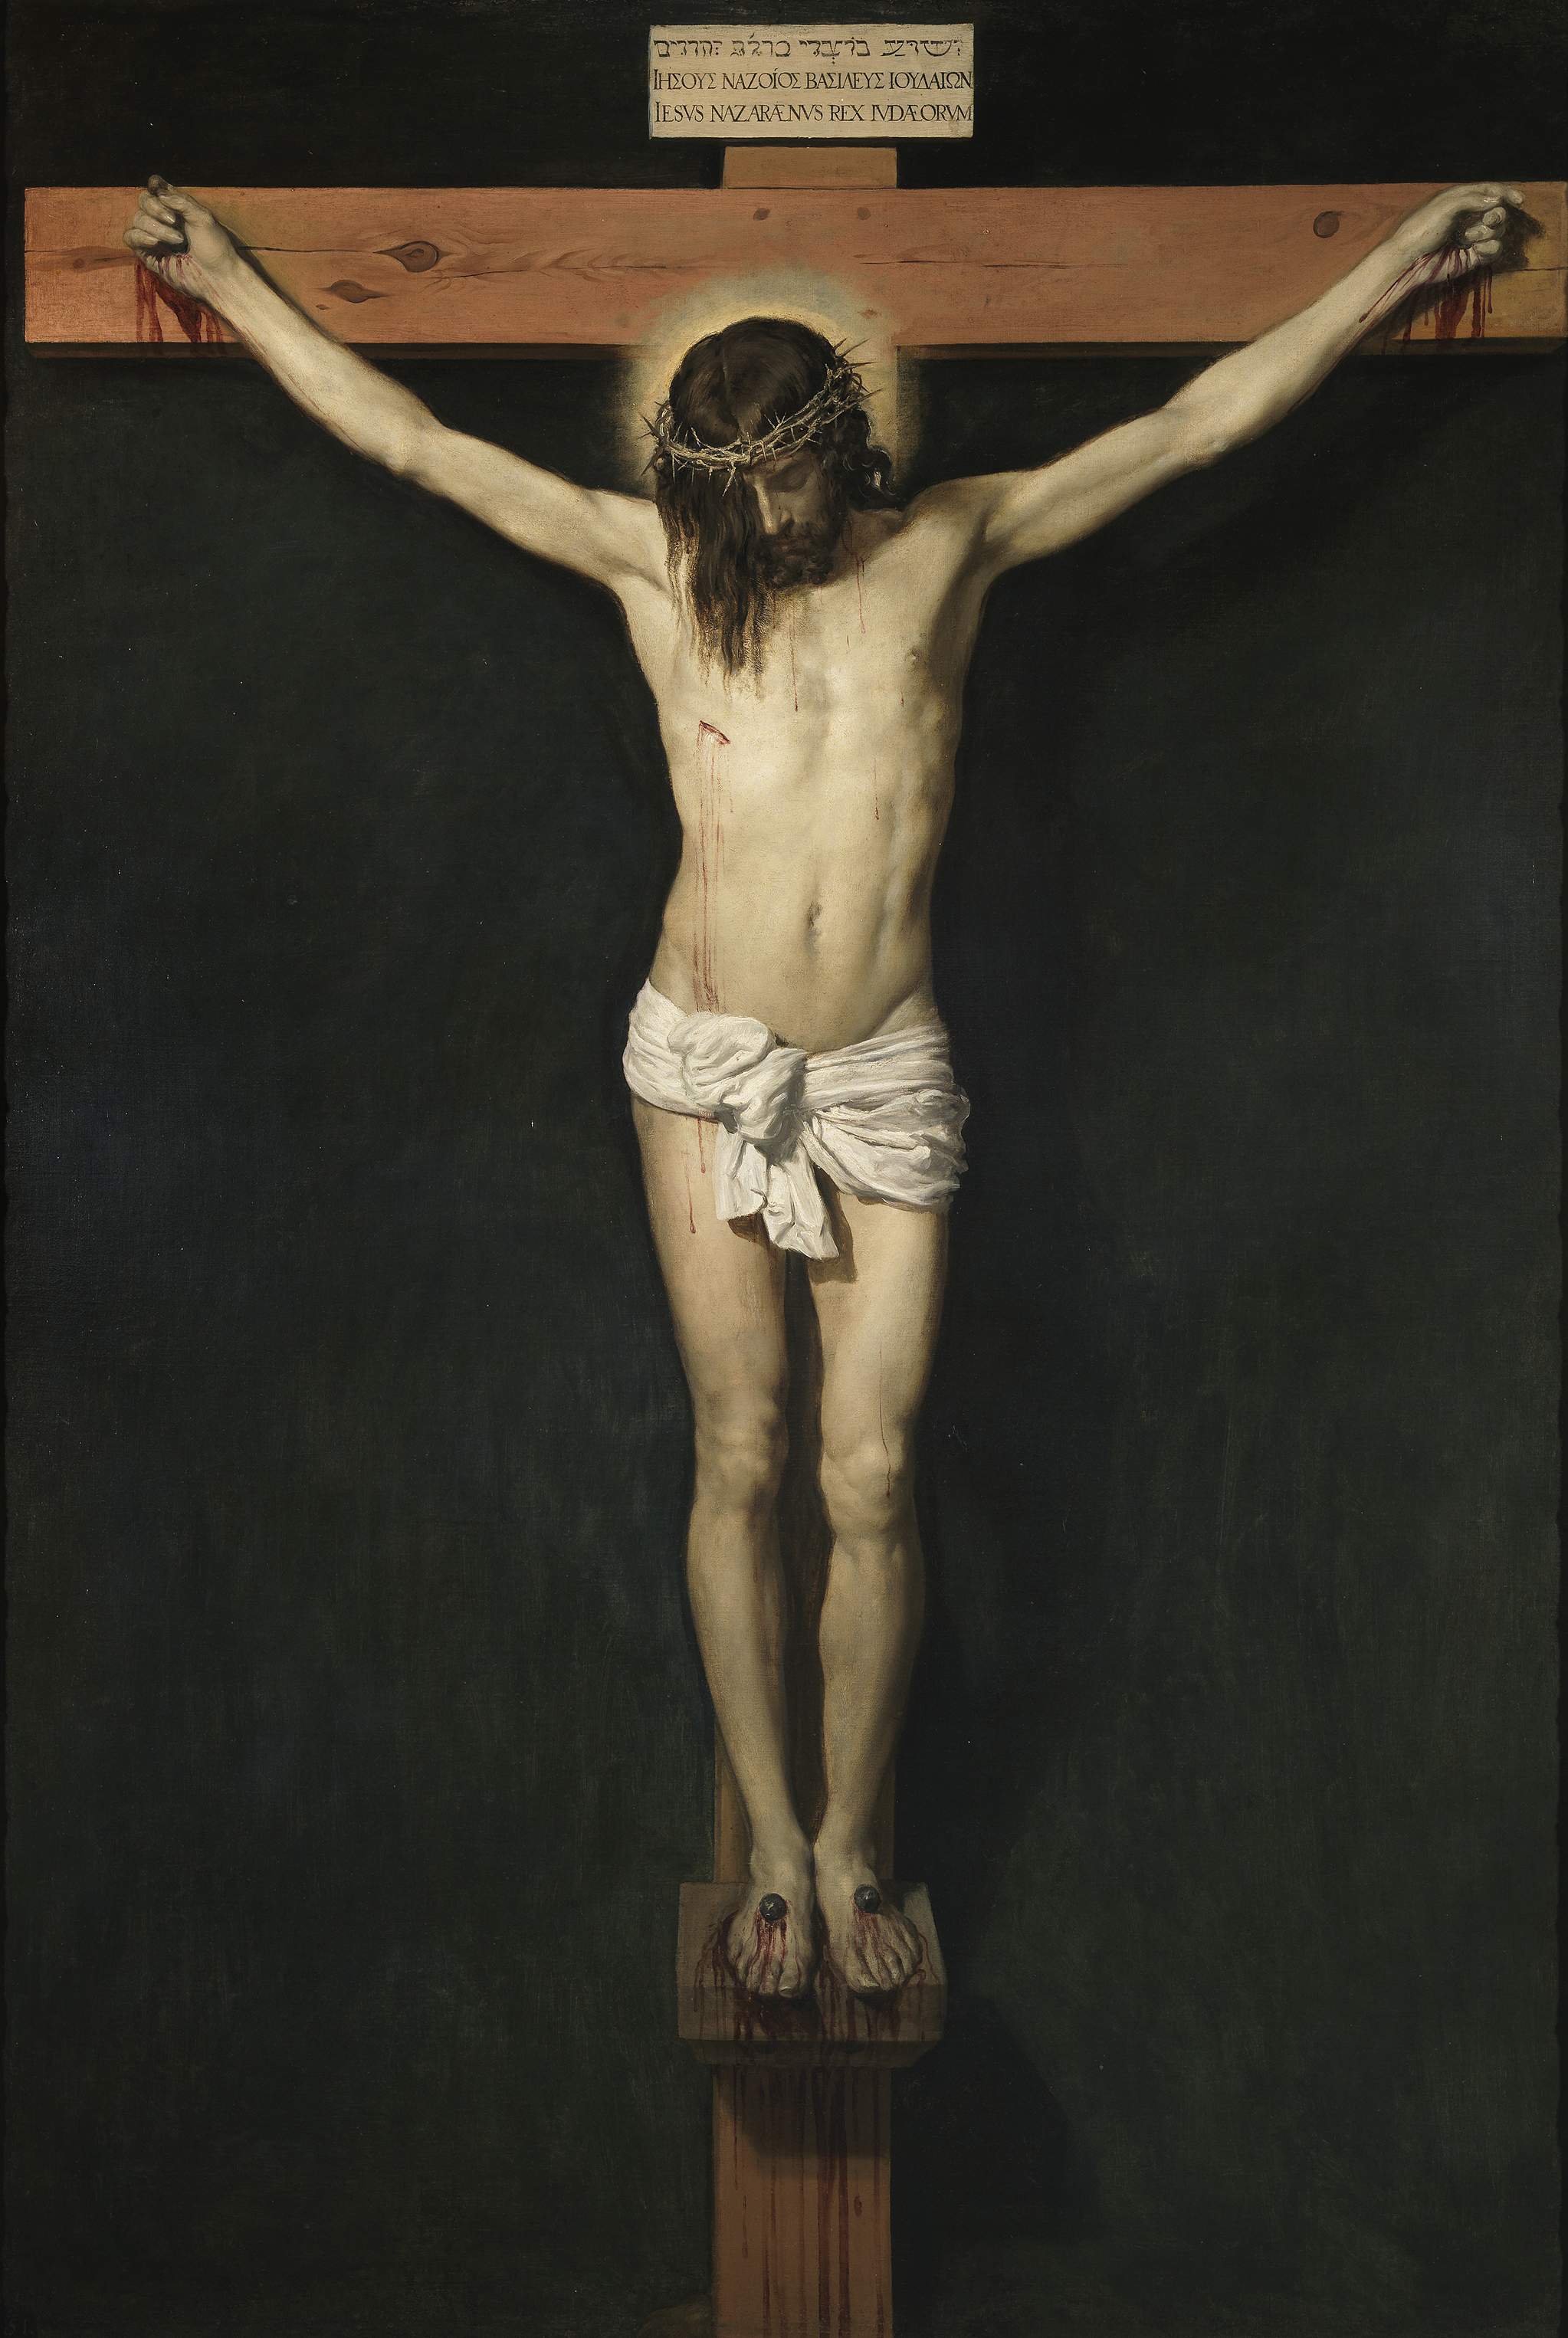
\includegraphics[width=1.0\textwidth]{velazquez.jpg}
%   .\caption{Cristo crucificado de Velázquez. Museo nacional del Prado} %. URL: www.museodelprado.es/coleccion/galeria-on-line/galeria-on-line/zoom/1/obra/cristo-crucificado-1/oimg/0/}
%\end{figure}

\newpage

\begin{description}
\item[Estilo] Actual
\item[Cronología] 2009-2010
\item[Lugar] 
\item[Autor] Juan Manuel Miñarro
\item[Título] Cristo de la Síndone o Sindónico
\end{description}

\textbf{Contexto histórico:} Esta obra es finalizada en 2010, tras más de nueve años empleados por el autor en su elaboración. El autor pretende mostrar lo más fielmente y científicamente posible la realidad de la muerte de Cristo. Se basa, por tanto, en una de las reliquias más conocidas, junto con el sudario de Oviedo, que posee relación con la muerte de Cristo: la Síndone de Turín o Sábana Santa, realizando mediante el estudio meticuloso de ésta una impresionante escultura.

Aunque no está demostrado científicamente que la Síndone fuese la sábana que envolvió a Cristo tras su muerte, presenta ciertas características que han hecho que los expertos y estudiosos de todo el mundo la identifiquen como tal. Una característica que contribuye a ello es la propia imagen que conserva grabada, que por un lado posee las características propias de un hombre torturado y crucificado de la misma forma que Cristo según los evangelios, y que por otro lado se considera imposible de falsificar con las técnicas de las que se disponen hoy en día y más difícilmente aún en cualquier época anterior, puesto que es algo no se puede crear ni de forma natural ni de forma artificial.

En su búsqueda de la realidad el autor refleja de forma impecable las heridas, contusiones, laceraciones y demás aspectos que proveen a la obra de un dramatismo nunca visto hasta ahora en la muerte de Cristo ni en obras pictóricas ni escultóricas. Además plasma todos aquellos detalles que identifican a Cristo como un hombre torturado a la hora de su muerte.

\vspace{12pt}
\textbf{Anatomía de superficie:}

En esta obra se nos muestra a un Cristo muy estudiado desde absolutamente todas y cada un de las perspectivas desde las que se puede tener en cuenta: en su anatomía, en la reproducción de la muerte y en la representación de las heridas y contusiones.

Al centrarnos en el primer punto se puede observar una figura proporcionada, y anatómicamente coherente con el conocimiento anatómico actual y con la imagen de la Síndone, mediante la cual el autor ha logrado producir la silueta y los detalles de Cristo en su muerte de una forma realista.

Además, el autor refleja con gran detalle las lesiones de Cristo.

Podemos apreciar los hasta 120 latigazos de los que fue víctima antes de ser crucificado y que están grabados con todo detalle en la piel de esta figura.

En el rostro presenta un gran hematoma en el lado derecho, que se extiende desde debajo del arco cigomático hasta el ojo. Presenta también una rotura del tabique nasal. Ambas lesiones pudieron deberse a los puñetazos que le pegaron ante Caifás antes de ser condenado, o una bofetada según dice el evangelio de Juan (Jn 18, 22; Lc 22, 63; Mc 14, 65; Mt 26, 67).

En la frente el autor nos muestra las heridas de la corona de espinas que continúan hacia la zona occipital de la cabeza, aunque son menos apreciables al estar cubiertas por el cabello.

Los orificios provocados por los clavos pueden apreciarse en ambas muñecas, en la región carpiana, según la creencia actual, en lugar de en las palmas de las manos. Y en los pies, que se cree que fueron clavados juntos con un solo clavo, debido a las características que presenta la Síndone, los orificios se encuentran en el punto de confluencia del calcaneo, astrágalo, escafoides y cuboides.

Así mismo el autor diferencia la proveniencia de la sangre, es decir, si Cristo todavía estaba vivo o si, por el contrario, ya estaba muerto cuando se produjo cada herida. Por ejemplo, en la herida del costado derecho producida por la lanza y situada por el autor entre la quinta y la sexta costilla, refleja el aspecto que podría tomar una herida postmortem, apreciándose la sangre como una masa coagulada y separada parcialmente del plasma, éste un color más claro.

Claramente se trata de una figura que representa a Cristo muerto una vez producido el descendimiento de Cristo de la Cruz.

La figura mantiene una postura rígida provocada por el \textit{rigor mortis}, que se cree pudo empezar a originarse poco después de la muerte de Cristo, como ocurre en aquellas personas que han sido sometidas a grandes esfuerzos o actividad extenuante. De hecho es probable que el \textit{rigor mortis} comenzase cuando Cristo aún se encontraba suspendido en la cruz. Por ello podemos observar que las extremidades inferiores conservan la posición en la que estarían en ese momento.

Sin embargo la posición de los brazos no es la que tendría un crucificado que ha permanecido en la cruz durante el \textit{rigor mortis}: brazos casi completamente extendidos, en abducción y supinación del antebrazo, por lo que se asume que las extremidades superiores fueron forzadas antes de producirse el \textit{rigor mortis} completo, momento en el que la movilización de éstos habría sido imposible sin desgarrar tejidos.

El crucificado muestra en las plantas de ambos pies un característico color azulado característico del \textit{livor mortis}. Éste consiste precisamente en la acumulación de la sangre por el efecto de la gravedad en las partes inferiores del cuerpo, según la posición de éste, proporcionando a la vez un color amarillento-ceniciento al resto del cuerpo por el que la sangre ya no fluye debido a la ausencia de latido cardíaco.

La figura estudiada demuestra que Cristo se mantuvo en la cruz después de muerto el tiempo suficiente como para que la sangre por efecto de la gravedad quedase retenida en la zona inferior de los miembros inferiores. Aunque no demasiado tiempo, pues en tal caso la cantidad de sangre acumulada en las extremidades inferiores sería superior, aun teniendo en cuenta la abundante sangre perdida antes y durante la crucifixión.

Además, queda patente que el cuerpo no ha permanecido en decúbito supino durante largo tiempo, ya que en tal caso la sangre también se habría acumulado en las zonas inferiores, en este caso la parte posterior de la figura.



Además, la figura no muestra la lividez típica de un cadáver, todo lo contrario, la figura posee el color de una persona totalmente sana, a pesar de la pérdida de sangre que Cristo debió experimentar durante su calvario. Otro detalle importante de la obra es la escasa sangre que emana de las heridas de Cristo: apenas varias gotas en las heridas de los clavos y aún menos en la herida de lanza que muestra en el costado derecho. Un rasgo de la obra que  manifiesta la muerte de Cristo, que como ya he dicho para nada está representada, es precisamente esta herida del costado, la cual en teoría fue realizada postmortem, como verificación de la muerte.

Una serie de músculos colaboran en la consecución de la postura en la que se encuentra la figura a analizar.

La espalda se encuentra erguida, los músculos que se encargan de mantener esta postura son los principales erectores de la columna: los músculos del grupo iliocostal, los del grupo longuísimo y los del espinoso.

El músculo dorsal ancho, que además se puede apreciar en la obra, proviene de la espalda e inserta en el ángulo inferior de la escápula. Su tendón estrecho envuelve al músculo redondo mayor que forma el pliegue posterior de la axila. Ambos músculos junto con el pectoral mayor, el que además forma el pliegue anterior de la axila, elevan el tronco cuando los brazos se encuentran fijos, como es el caso de la figura examinada.

El músculo trapecio, cuya principal función es la elevación de la escápula, también se observa. El serrato anterior gira la escápula y, por tanto, junto con el músculo trapecio y el elevador de la escápula que la elevan hacen que la cavidad glenoidea se oriente hacia arriba y adelante, como en la figura de la obra de Velázquez.
El deltoides, que se ve fácilmente redondeando y sustentando la articulación del hombro por su parte superior, es el principal abductor del brazo, ya que sigue el movimiento abductor que el músculo supraespinoso inicia, por lo que tiene gran relevancia en la posición de crucifixión en la que ambos brazos se encuentran en posición de abducción.

En el brazo se observan tanto el bíceps como el tríceps. El bíceps forma una prominencia en la parte anterior del brazo y se encarga de la supinación del antebrazo, la cual realiza con la ayuda del músculo supinador. El tríceps por su parte se encarga de la extensión de la articulación del codo. En este movimiento le secunda el músculo ancóneo, que no es visible en la figura de la obra analizada por encontrarse en la parte posterior del codo.

La mano se encuentra en posición de reposo en la que las articulaciones falángicas y metacarpofalángicas se encuentran ligeramente flexionadas. El músculo palmar largo contribuye sutilmente a la flexión de las articulaciones metacarpofalángicas, que es realizada fundamentalmente por los músculos flexores de los dedos.

Al tratarse de un individuo delgado y favorecido por la postura en que se encuentra (brazos estirados hacia los lados y hacia arriba) se puede intuir la caja torácico perfectamente. El borde costal inferior formado por las seis últimas costillas es fácilmente visible, al igual que la depresión en la que se encuentra el cuerpo del esternón y el contorno de algunas costillas (probablemente la cuarta, quinta, sexta y séptima).

En el abdomen se encuentran los músculos abdominales, que se pueden apreciar, aunque no muy marcados. Estos músculos forman una vaina fibrosa a cada lado de la línea media. Ambas vainas se unen en esta, formando la línea alba. También se divisa bastante bien la línea semilunar, que marca el borde lateral del músculo recto del abdomen cuya principal función en la figura es el mantenimiento de la postura erecta apoyando así a los músculos erectores de la columna.

El músculo mas superficial de los músculos laminares del abdomen es el oblicuo externo. Este entre la espina y la tuberosidad púbica gira sobre sí mismo y forma el ligamento inguinal. La depresión que suele haber a la altura de ese ligamento, y que suele ser más visible en hombre, se puede observar perfectamente en la obra pictórica.

La posición de las piernas, en las que la rodilla derecha de la figura se encuentran una en posición de extensión, mientras que la otra se encuentra ligeramente flexionada, colaboran varios músculos. Los encargados de la extensión son: el cuadriceps y los músculos del tracto iliotibial, y los de la flexión son: los músculos poplíteos y los gemelos. Al estar de pie soportando el peso sobre una pierna, el lado de la pelvis que no soporta el peso se eleva. Esta acción está realizada por los glúteos medio y menor y deja a la vista la espina ilíaca del lado derecho.
La rótula o patella se puede apreciar, al igual que la tuberosidad tibial, sobre todo en la rodilla flexionada.

Los pies se encuentran apoyados en una tabla, soportando el peso del cuerpo, y se ubican en paralelo entre ellos ligeramente separados anteriormente, con un clavo en cada dorso y sangre que emana de la herida. En la parte anterior de éstos, los dedos se encuentran relajados..
\section{Resultados y discusión}

Se han obtenido resultados según los objetivos planteados en el apartado en el que se establecen estos. Han sido logrados mediante la búsqueda de información en diversas fuentes y la selección, a su vez, de la información relevante en el tema a desarrollar.

En cuanto a la información encontrada, se ha buscado en fuentes de datos fiables, siendo ésta de buena calidad en su mayoría. El mayor problema en la búsqueda de información ha sido la búsqueda en las bases de datos de aquellos documentos o artículos en los que, después de haberlos encontrado, no aparece el texto, mostrándose sólo el nombre del autor y el título, sin posibilidad de disponer de él para adquirir información. Este problema ha sido contrarrestado parcialmente gracias a la página web de la biblioteca de la Universidad del País Vasco / Euskal Herriko Unibertsitatea.

En algunos casos la información se contradice, es el caso, por ejemplo, de la localización de los clavos de las extremidades superiores en la crucifixión. En este tema existen experimentos en los que se muestra que un crucificado no podría mantenerse sujeto a la cruz mediante la inserción de los clavos en las palmas de las manos, mientras que otros estudios dicen que si es posible al tener ambos pies también sujetos y no colgando. Aún así, y después de leer la limitada bibliografía que existe acerca de ello parece que la hipótesis más extendida es la de que los clavos se encontraban a la altura de las muñecas.

Sobre este mismo tema acerca de la crucifixión de Cristo y las causas de su muerte no existen numerosos artículos que lo amplien, sí que he podido encontrar varios en los que se habla de las distintas hipótesis que se manejan, no sacando en claro cuál es la más fidedigna. Por ello he dejado constancia de todas aquellas posibilidades de acuerdo con el estudio científico tanto de lo mencionado en la Biblia como de otras crucifixiones conocidas.

En otros apartados del trabajo no ha habido tanto problema para la obtención de información, la cual, sin embargo, ha tenido que ser resumida y acotada al tema relevante. Es el caso de la historia de la anatomía en la que existen numerosos documentos, sobre todo acerca de Andrea Vesalio.

Refiriéndome al tema principal del trabajo, he de admitir que la anatomía de superficie no es un tema del que haya podido obtener mucha información. Empezando por la propia definición del término: tras haber leído una cantidad no muy extensa de definiciones, ninguna que me complaciese del todo, he decidido hacer una propia basándome en las anteriormente leídas.

Para analizar la anatomía de superficie de las obras pictóricas analizadas, al final he tenido que recurrir a un libro que se centraba en esta desde un punto de vista totalmente médico, habiéndole añadido yo la parte artística según mi propio conocimiento e ingenio. Sin embargo la parte artística de las obras está perfectamente documentada en diferentes libros y páginas de internet.

En general y tras diversas dificultades %que he encontrado por el camino, 
creo que he llegado a cumplir la mayor parte de los objetivos formulados, desarrollando un TFG interesante y muy trabajado.
\section{Conclusión}
Tras haber realizado el análisis de varias obras de distintas épocas se pueden sacar varias ideas en claro.

Las obras se rigen por el estilo predominante de la época, aunque en ocasiones los autores de éstas aporten novedades en el arte de su tiempo, como Mantegna que revolucionó la perspectiva con su lamentación sobre Cristo muerto o Dalí con su estilo único.

La intención del autor también cambia. Algunos autores intentan mostrar una obra bella utilizando para ello proporciones y armonía, como Velázquez o Dalí, mientras que otros utilizan la prevalencia del realismo para crear una obra que represente la muerte de Cristo de una forma lo más exacta a la posible realidad, éste es el caso de Mantegna o Miñarro.

En relación a la anatomía, %se ve diferencia entre aquellas obras anteriores a las disecciones del cuerpo y aquellas en las que el conocimiento del cuerpo era mayor.
la figura de la obra de Mantegna posee una anatomía estudiada, sin embargo no es en lo que más se centra, numerosos detalles en la obra son más impresionantes, como la perspectiva que adopta la figura de Cristo o los rasgos referentes a la muerte que éste presenta. Velázquez sí que se centra mucho en la anatomía superficial y en las proporciones del Cristo de su obra. Dalí, por su parte, se propone dibujar el Cristo más bello, para el que adopta una perspectiva nueva e incluso se dice que utiliza un modelo para representar de forma correcta la anatomía. Miñarro, por su parte, se basa en la Síndone de Turín para intentar representar la muerte de Cristo como nunca hasta ahora se había visto, en toda su crudeza.

%El número de clavos con el que Cristo aparece clavado en la Cruz es variable debido, más a las ideas del propio autor que a las de la época. De hecho, en todas las obras analizadas se puede observar la inserción de tres clavos, uno uniendo los dos pies y otro en cada extremidad superior, excepto en la obra de Velázquez que se deja influir por su maestro, y no así por su tiempo. Otro detalle sobre la inserción de los clavos es que a lo largo del tiempo el Evangelio de San Juan ha sido interpretado de forma que incluso en épocas más modernas estos se han seguido representado en la palma de la mano y no ha sido hasta hace varias décadas que se han hecho experimentos en cuanto a ello. Por ello, en la obra de Miñarro es en la única que se pueden apreciar los clavos a la altura de los carpos y no entre los metacarpos como se representa en las demás obras.

En cuanto a la representación de la muerte de Cristo, Mantegna en su obra presenta la laxitud en la postura y la rigidez en algunos músculos, que probablemente está relacionada con el \textit{rigor mortis}, además de la lividez con la que el autor ilustra el cuerpo, reproduciendo de manera bastante acertada la apariencia de un cadáver.

Velázquez, sin embargo, realiza una obra en la que no reproduce la muerte de Cristo. El Cristo no posee ninguna característica de un cuerpo muerto, ni laxitud en los músculos ni lividez cadavérica. Es más, muestra ciertas características que nos llevan a la conclusión de que el Cristo no ha fallecido e icluso se encuentra en relativas buenas condiciones, sobre todo, tratándose de una figura que ha soportado toda clase de martirios.

Dalí propone la imagen de un Cristo que no porta nungún elemento utilizado para su suplicio ni crucifixión. Aún así, nos muestra una cristo cuyos músculos están relajados, como si estuviese a punto de fallecer o ya hubiera fallecido. En cuanto a la coloración del cuerpo, es dificil de determinar si posee la coloración característica del \textit{livor mortis} o no, debido al gran contraste de luz que Dalí utiliza en la obra.

En el Cristo de la Síndone de Miñarro se distinguen fácilmente las características de la muerte en la figura. De hecho ésta posee un \textit{rigor mortis} con una rigidez muy marcada y un \textit{livor mortis} que se aprecia en el color ceniciento del cuerpo, así como en el acúmulo de sangre en la zona más distal de las extremidades inferiores.

\nocite{*} % Show all Bib-entries
\bibliographystyle{myvancouver}
\bibliography{bibliography}

\clearpage
\begin{appendices}
\let\clearpage\relax
\section{Tipos de Cruces} \label{app:crosses}
Tradicionalmente existe cuatro tipos de cruces según su morfología específica básica. Estos cuatro modelos son:
%\begin{itemize}
%\item[La cruz Latina, cruz immissa o cruz ordinaria]
%\item[La cruz Griega o cruz immissa quadrata]
%\item[La cruz de San Andrés o cruz decussata]
%\item[La cruz Tau, cruz commissa o en forma de T]
%\end{itemize}

\begin{description}
\item[] La cruz Latina, cruz \textit{Immissa} o cruz ordinaria
\item[] La cruz Griega o cruz \textit{Immissa quadrata}
\item[] La cruz de San Andrés o cruz \textit{Decussata}
\item[] La cruz Tau, cruz \textit{Commissa} o en forma de T
\end{description}


\begin{figure}[ht!]
    \centering
    \includegraphics[width=1\textwidth]{cruces.jpg}
    \caption{URL:http://www.crosses.org/history.htm}
\end{figure}
\end{appendices}

\end{document}
